\Chapter{Tesztelés}

Ebben a fejezetben a Backend teszteléséről lesz szó. A teszteléshez a Postman-t alkal-
mazást használtam.

\Section{Regisztráció szimuláció}

\subsection{Helytelen Jelszó}

Ebben a szimulációban jelszó nélkül szeretnénk regisztrálni. Eredménye:"2" lesz.
\begin{figure}[h]
\centering
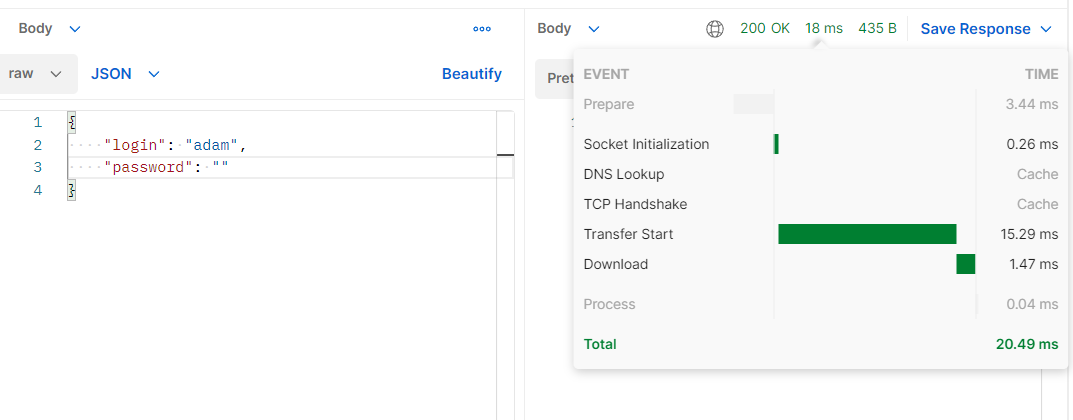
\includegraphics[scale=0.6]{images/Hibas_regisztracio.png}
\caption{Jelszó nélküli regisztráció}
\label{fig:JWT}
\end{figure}

\subsection{Sikeres Regisztráció}
Ebben a szimulációban egy sikeres regisztráció fog végbe menni Eredménye:"Valamelyik mezőt kitöltettlenül hagyta!" lesz.
\begin{figure}[h]
\centering
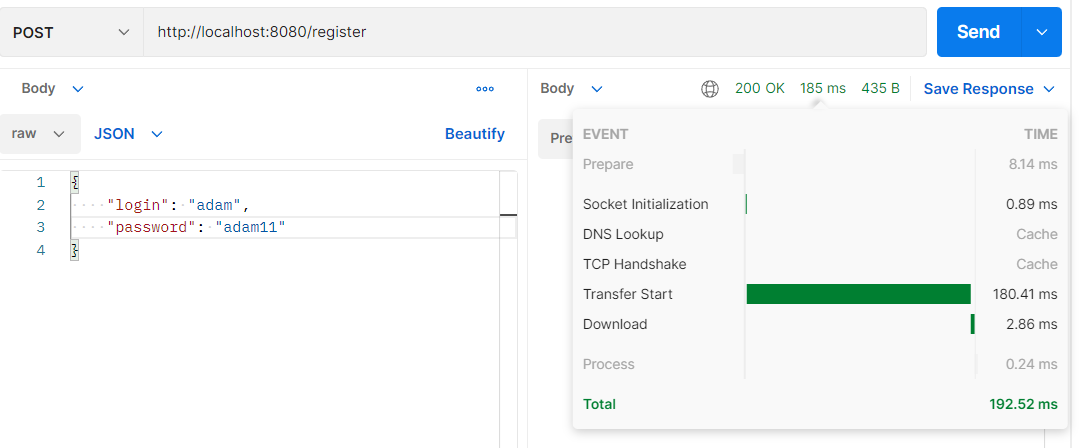
\includegraphics[scale=0.6]{images/Sikeres_regisztracio.png}
\caption{Sikeres Regisztráció}
\label{fig:JWT}
\end{figure}